\documentclass[12pt,a4paper]{article}


\newcommand{\AppName}{Maxwell Bloch Studio}
\newcommand{\AppVersion}{10.0.6}
  % written from pyproject.toml by tools/build_docs.sh
\newcommand{\AppAuthor}{Vahid Anari}
\newcommand{\AppEmail}{vahid.anari8@gmail.com}
\newcommand{\DocName}{User Guide}
\usepackage{style}

% ── Convenience macros ────────────────────────────────────────────────────────
\newcommand{\tab}[1]{\textbf{#1}}
\newcommand{\menu}[1]{\texttt{#1}}
\newcommand{\param}[1]{\textit{#1}}
\newcommand{\key}[1]{\texttt{#1}}
\newcommand{\T}{T_0}
\newcommand{\mb}{Maxwell--Bloch}
\newcommand{\sech}{\operatorname{sech}}
\newcommand{\pderiv}[2]{\dfrac{\partial #1}{\partial #2}}
% ══════════════════════════════════════════════════════════════════════════════
\begin{document}

% ── Title page ────────────────────────────────────────────────────────────────
\begin{titlepage}
  \centering
  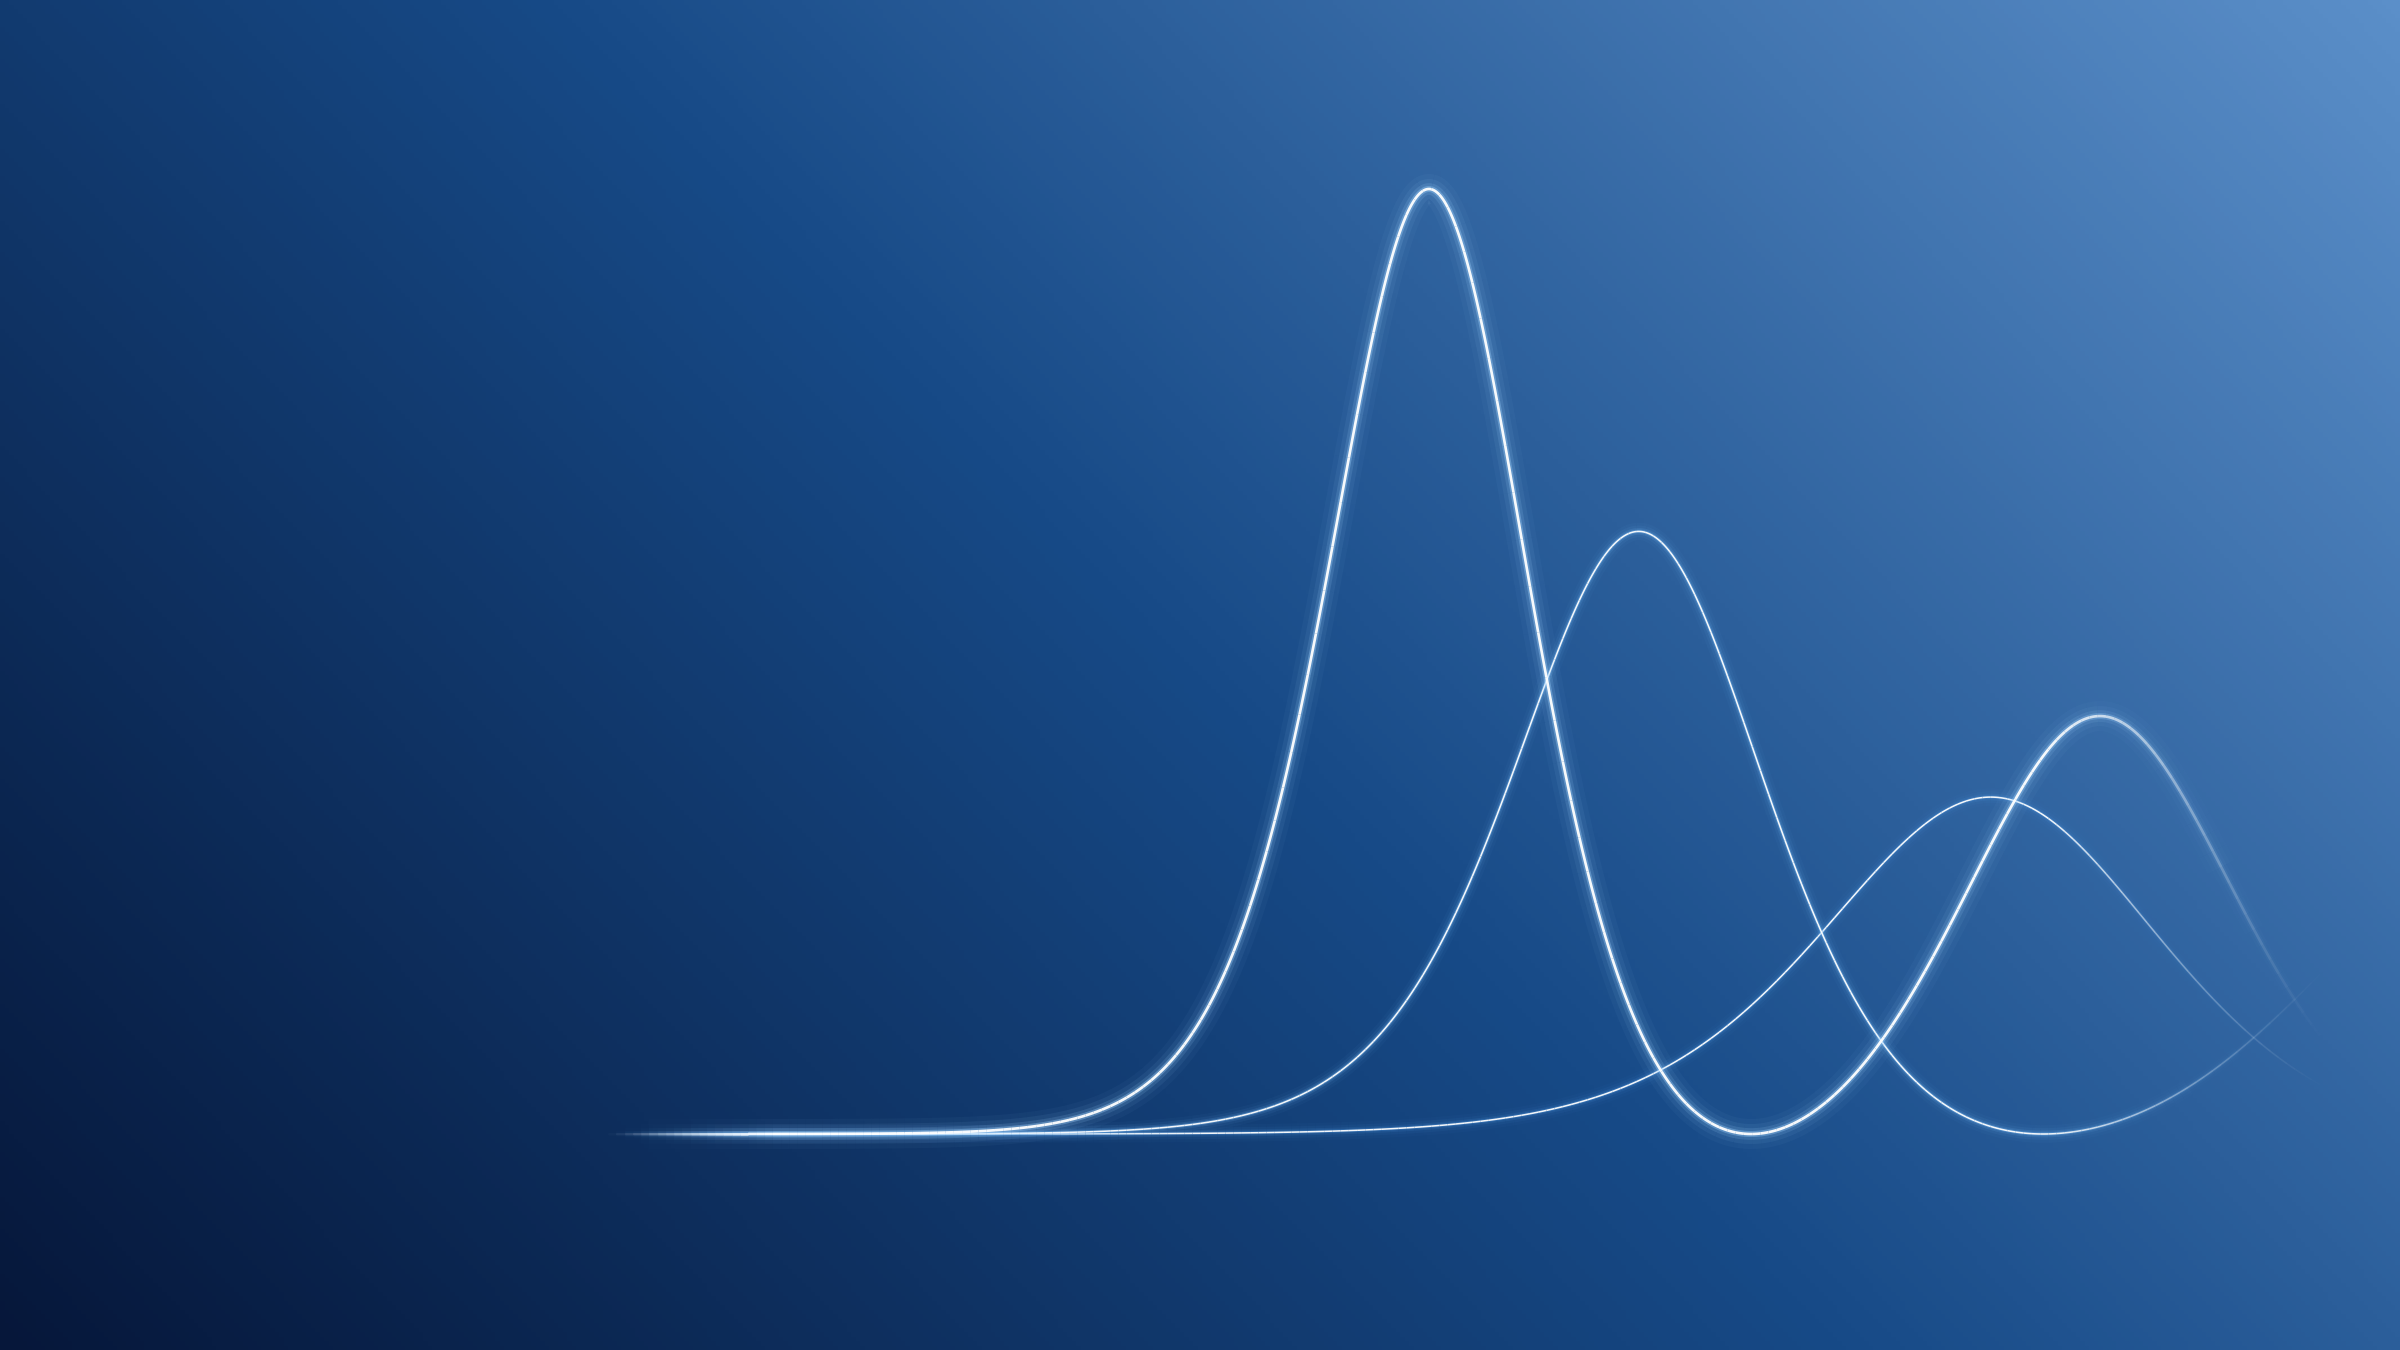
\includegraphics[width=\textwidth,trim=180 0 0 0,clip]{figures/splash.png}\\[2cm]
  {\Huge\bfseries\color{accent} \AppName}\\[0.5em]
  {\large \DocName}\\[0.3em]
  {\normalsize Version \AppVersion}\\[3cm]

  {\large \AppAuthor}\\[0.4em]
  \href{mailto:\AppEmail}{\texttt{\AppEmail}}\\[3cm]

  \vfill
  {\small\color{gray} This document describes the interactive desktop application
  for solving the Maxwell--Bloch equations, exploring driven coherent radiative
  regimes, and comparing model results with astronomical light curves.}
\end{titlepage}

\tableofcontents
\newpage

% ══════════════════════════════════════════════════════════════════════════════
\section{Overview}

\textbf{\AppName} is a desktop GUI application for numerically solving the
\mb{} equations and visualizing the resulting intensity, inversion, pump, boundary-field,
and relaxation-time profiles. The app is intended for coherent-radiation problems in which a driven resonant medium
is modeled with a one-dimensional Maxwell--Bloch system.

In astrophysical work, the same framework can be used to study several regimes, including:
\begin{itemize}[noitemsep]
  \item steady or slowly varying \textbf{maser} amplification,
  \item transient \textbf{superradiant} bursts,
  \item weakly radiative or suppressed-response regimes that may be interpreted as
  \textbf{subradiant} behaviour depending on the chosen initial conditions and relaxation times.
\end{itemize}

The application provides:
\begin{itemize}[noitemsep]
  \item interactive parameter editing with sliders, line edits, and combo boxes,
  \item automatic re-solving when physical solver parameters change,
  \item two operating modes: \textbf{standalone simulation} and \textbf{fit mode},
  \item overlay of simulation results with observational light curves,
  \item JSON-based parameter/configuration saving,
  \item export of the current figure to PDF, PNG, or SVG,
  \item a PDF export report containing metadata and the current parameter state.
\end{itemize}

\begin{notebox}
The app is designed around fast interactive exploration. In normal use, there is no separate
``Run'' button: changing a solver parameter triggers a new solve automatically.
\end{notebox}

% ══════════════════════════════════════════════════════════════════════════════
\section{Physical Model}
\label{sec:model}

The solver evolves a dimensionless one-dimensional Maxwell--Bloch system
for a driven two-level medium. The equations solved by the application are
\begin{align}
  \pderiv{w}{\tau'}
    &= A'R - \frac{w - w_0}{T_1'} + \Lambda_n',
  \label{eq:realw}\\[8pt]
  \pderiv{R}{\tau'}
    &= -A'\,w - \frac{R - R_0}{T_2'},
  \label{eq:realR}\\[8pt]
  \pderiv{A'}{z'}
    &= -\eta\, R,
  \label{eq:realA}
\end{align}
where $w$ is the population inversion, $R$ is the medium coherence, and
$A'$ is the dimensionless field envelope. The solver works in normalised
variables, with $\tau' = \tau/\T$ and $z' = z/L$ a propagation coordinate
normalised to the sample length $L$.

\begin{center}
\begin{tabular}{@{}ll@{}}
  \toprule
  Symbol & Meaning \\
  \midrule
  $w(\tau',z')$              & Population inversion $\rho_{22}-\rho_{11}$ \\
  $R(\tau',z')$              & Coherence envelope ($\rho_{21} = \tfrac{1}{2}R\,e^{i(kz-\omega t)}$) \\
  $A'(\tau',z')$             & Dimensionless field envelope \\
  $\tau' = \tau/\T$          & Normalised retarded time \\
  $z' = z/L$                 & Normalised propagation distance \\
  $T_1' = T_1/\T$            & Longitudinal relaxation time (may vary with $\tau'$) \\
  $T_2' = T_2/\T$            & Transverse dephasing time (may vary with $\tau'$) \\
  $\eta = \T/T_R$            & Dimensionless coupling parameter \\
  $\Lambda_n' = \T\Lambda_n$ & Dimensionless pump rate \\
  $w_0,\,R_0$                & Equilibrium inversion and coherence \\
  \bottomrule
\end{tabular}
\end{center}

The physical reference time $\T$ is set in the \tab{Sample} tab.
By default, $\T = 86400\,\mathrm{s}$ (one day), but any positive value
may be used. The derivation of these equations from first principles is
given in the companion Equations Reference document.
\subsection{Numerical Method}

The application solves the system numerically on a time--space grid. The matter variables are advanced
in time with a fourth-order Runge--Kutta scheme, while the field is propagated through the spatial grid.
Performance-critical loops are accelerated with Numba.

\subsection{Input Profiles}
\label{sec:profiles}

The boundary field, the pump, and the relaxation times are entered as
time profiles. Two profile types are used.

\subsubsection*{Pulse profiles (boundary field and pump)}

The boundary field $A'\vert_{z'=0}$ and each pump contribution are sums of
$N$ $\sech^2$ pulses,
\begin{equation}
  f(\tau') = \sum_{i=0}^{N-1} a^i\,\sech^2\!\left(\frac{\tau'-\tau_0^{i}}{w^{i}}\right),
\end{equation}
with amplitude $a^i$, center $\tau_0^i$, and width $w^i$.

\subsubsection*{Step profiles (relaxation times)}

Each of $T_1'$ and $T_2'$ is either a constant or a sequence of smoothed
steps between $N$ levels $y^0, \dots, y^{N-1}$,
\begin{equation}
  y(\tau') = y^0 + \sum_{i=1}^{N-1}
  \frac{y^i - y^{i-1}}{2}
  \left[1 + \tanh\!\left(\frac{\tau'-\tau_0^i}{w^i}\right)\right].
\end{equation}
Step $i$ switches from $y^{i-1}$ to $y^i$ around $\tau_0^i$, over a time
of order $2w^i$. With $N = 1$ the profile is the constant $y^0$.

\subsubsection*{Common options}

In asymmetric mode, both profile types use separate widths on each side of
the center,
\begin{equation}
  w^i =
  \begin{cases}
    w_l^i, & \tau' < \tau_0^i,\\
    w_r^i, & \tau' > \tau_0^i.
  \end{cases}
\end{equation}

An optional spacing control places the centers at regular intervals of
$\tau_p$:
\begin{equation}
  \tau_0^i = \tau_0^0 + i\,\tau_p \quad\text{(pulses)},
  \qquad
  \tau_0^i = \tau_0^1 + (i-1)\,\tau_p \quad\text{(steps)}.
\end{equation}
This is useful for repeated pulses or regularly spaced changes.
% ══════════════════════════════════════════════════════════════════════════════
\section{Getting Started}

\subsection{Launching the Application}

Install the application once with
\begin{verbatim}
pipx install maxwell-bloch-studio
\end{verbatim}
(or \texttt{pip install maxwell-bloch-studio} inside a conda or virtual environment),
then start it with
\begin{verbatim}
maxwell-bloch-studio
\end{verbatim}
or the shorter \texttt{mbstudio}. Until version 9 the application was called
Maxwell Bloch Solver; saved settings and parameter files carry over.
A splash screen appears during startup, followed by the main window.

\subsection{Command Line}\label{sec:cli}

The \texttt{mbstudio} command also works from a terminal:
\begin{center}
\begin{tabular}{@{}ll@{}}
  \toprule
  Command & Effect \\
  \midrule
  \texttt{mbstudio} & start the application \\
  \texttt{mbstudio PATH} & start it and open a parameter file or a data folder \\
  \texttt{mbstudio -{}-version} & print the versions of the app, solver, widgets and Python \\
  \texttt{mbstudio update -{}-check} & show whether a newer version exists, and what is new \\
  \texttt{mbstudio update} & update the app (asks first) \\
  \texttt{mbstudio solve FILE} & solve a parameter file without the window \\
  \texttt{mbstudio example [PATH]} & save the example script of Section~\ref{sec:python} \\
  \texttt{mbstudio -{}-help} & list all of this \\
  \bottomrule
\end{tabular}
\end{center}

\texttt{mbstudio PATH} opens a folder as a data folder (Section~\ref{sec:fitmode}); a
parameter file saved with a data folder opens that folder, and any other parameter file is
loaded as with \menu{File $\to$ Open Parameters...}.

\texttt{mbstudio update} finds out how the app was installed and runs
\texttt{pipx upgrade maxwell-bloch-studio} or \texttt{pip install -U maxwell-bloch-studio} in
the same Python; add \texttt{-{}-yes} to skip the question. A copy installed from a source folder
(\texttt{pip install -e}) is updated there with \texttt{git pull} instead.

\texttt{mbstudio solve FILE} computes the same numbers as the app and saves them to
\texttt{FILE\_results.npz} next to the file (\texttt{-o NAME.npz} or \texttt{-{}-output-dir DIR}
to choose). The file holds the arrays \texttt{time}, \texttt{intensity}, \texttt{w},
\texttt{lambda\_n}, \texttt{A0}, \texttt{t1}, \texttt{t2} (as in
Section~\ref{sec:python}) and the parameters as JSON text, \texttt{params}; read it with
\texttt{numpy.load}. For the parameter file of a data folder, choose a velocity with
\texttt{-{}-velocity 12.3}, or solve every velocity with \texttt{-{}-all}, one file each.
This runs on machines without a display, such as a computing cluster.

\subsection{Operating Modes}

The application has two main modes.

\begin{enumerate}[noitemsep]
  \item \textbf{Standalone simulation mode:} used when no data folder is loaded. The app solves the
  Maxwell--Bloch system directly from the current parameters.
  \item \textbf{Fit mode:} entered after loading a light-curve folder. In this mode, the top panel overlays
  observational data and the model curve for one selected velocity component.
\end{enumerate}

\subsection{Main Window Layout}

The main window is divided into three user-facing areas.

\begin{itemize}[noitemsep]
  \item \textbf{Top toolbar (fit mode only):} velocity navigation, save/unsave controls,
  an ``Only saved velocities'' filter, and a $\chi^2$-style mismatch readout.
  \item \textbf{Central plot area:} two vertically stacked panels that share the time axis.
  The top panel shows intensity or flux; the bottom panel shows one selected auxiliary curve.
  \item \textbf{Parameter tabs:} organized controls for the sample, solver grid, initial conditions,
  driving terms, fit alignment, and display ranges.
\end{itemize}

A selector labeled \textbf{Bottom Plot} appears beside the velocity controls and chooses which
auxiliary quantity is shown in the lower panel. The \textbf{w} check box next to it shows or hides
the population inversion on the panel's right axis. Both show each curve's colour.

Figure~\ref{fig:main-window} shows the window in standalone mode.
\begin{figure}[htbp]
  \centering
  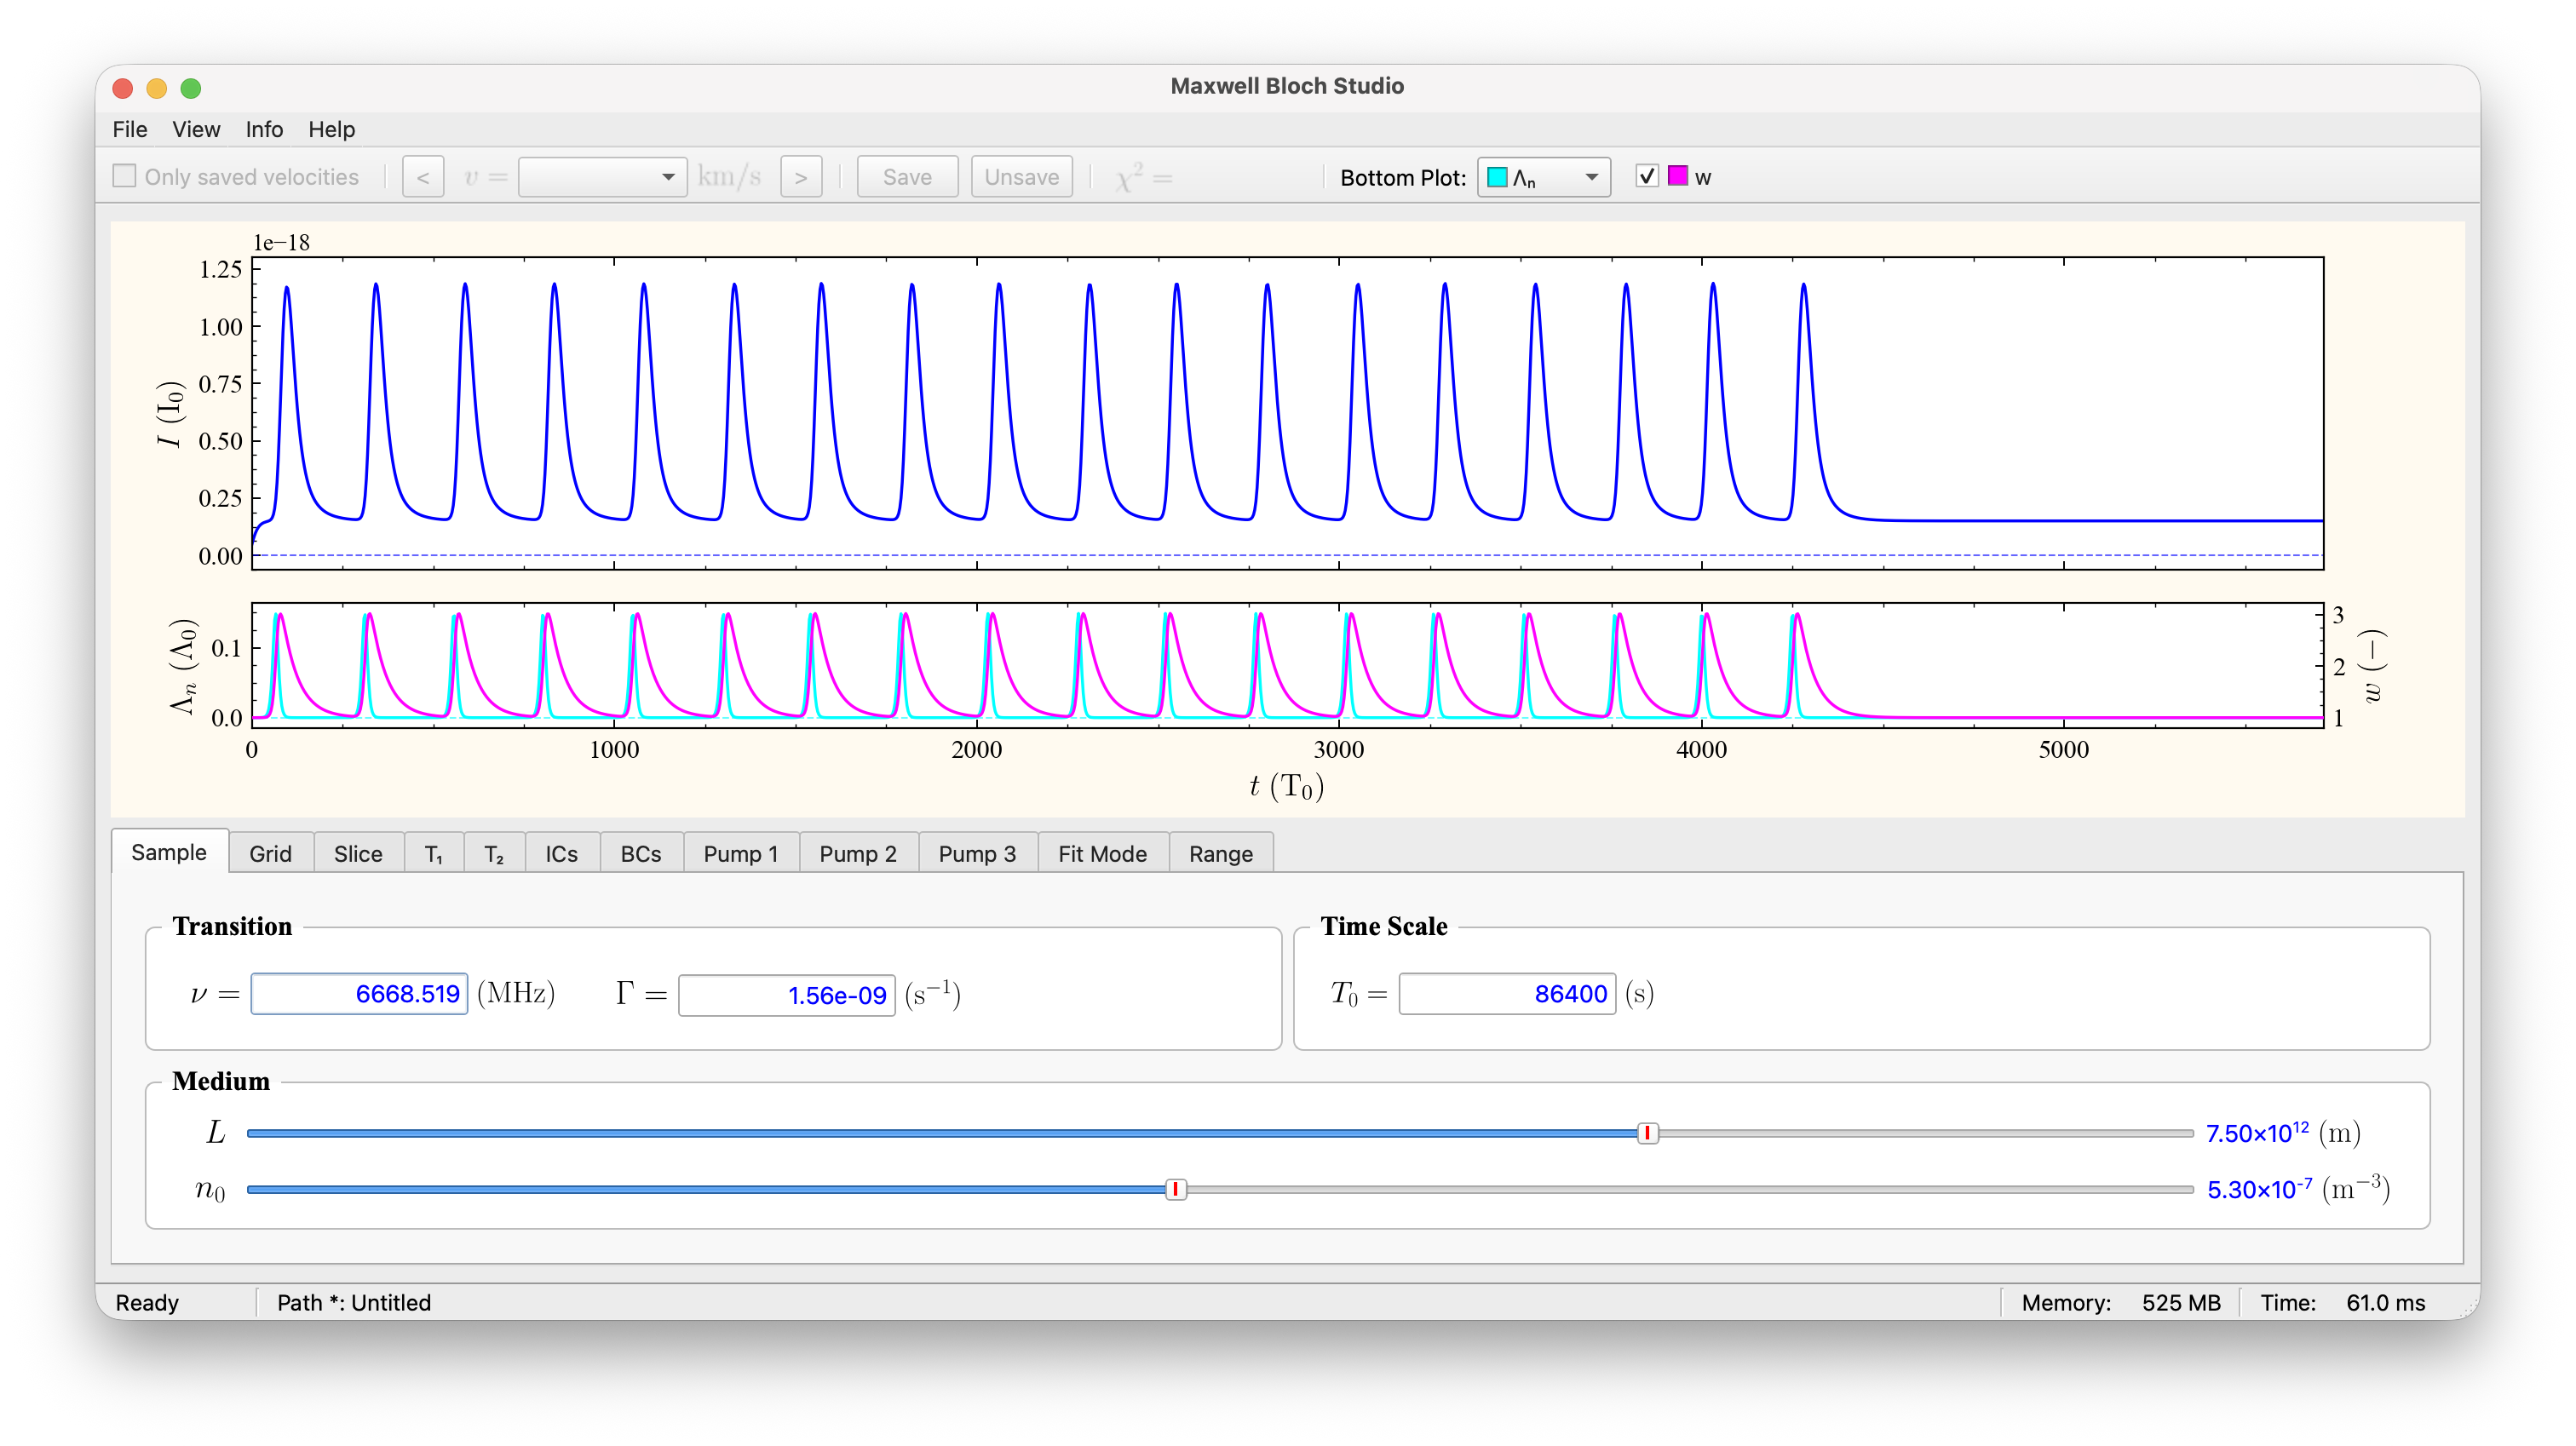
\includegraphics[width=\textwidth]{figures/main_window.png}
  \caption{The main window in standalone mode: plot area (top) and parameter tabs (bottom). The fit-mode toolbar is inactive.}
  \label{fig:main-window}
\end{figure}

% ══════════════════════════════════════════════════════════════════════════════
\section{Parameter Tabs}
\label{sec:tabs}

\subsection{Sample Tab}

The \tab{Sample} tab defines the global physical scaling:
\begin{center}
\begin{tabular}{@{}lll@{}}
  \toprule
  Parameter & Symbol & Description \\
  \midrule
  Transition frequency & $\nu$ & Line frequency \\
  Spontaneous emission rate & $\Gamma$ & Einstein-$A$-type rate \\
  Time scale & $T_0$ & Physical reference time \\
  Sample length & $L$ & Physical propagation length \\
  Number density & $n_0$ & Medium number density \\
  \bottomrule
\end{tabular}
\end{center}

From these values, the app derives internal scaling quantities such as the coupling constant $\eta$.
The expression used by the app can be viewed from \menu{Info $\to$ Scaling Formula}.

\subsection{Grid Tab}

The \tab{Grid} tab controls the numerical resolution:
\begin{center}
\begin{tabular}{@{}lll@{}}
  \toprule
  Parameter & Symbol & Description \\
  \midrule
  Time points & $N_t$ & Number of time-grid samples \\
  Spatial points & $N_z$ & Number of propagation steps \\
  Total time span & $T_{\max}$ & Simulation duration in units of $T_0$ \\
  \bottomrule
\end{tabular}
\end{center}

Increasing $N_t$ or $N_z$ generally improves resolution but also increases solve time.

\subsection{Slice Tab}

The \tab{Slice} tab selects which spatial position is shown in the plots.
The displayed solution is taken from one sampled $z$ plane within the interval $[0,1]$.
Changing only the selected slice updates the displayed curve immediately. If the underlying slice array
length is changed, the app performs a new solve.

\subsection{T\textsubscript{1} and T\textsubscript{2} Tabs}

The \tab{T\textsubscript{1}} and \tab{T\textsubscript{2}} tabs set the
longitudinal relaxation time $T_1$ and the transverse dephasing time $T_2$,
in units of $T_0$. Each uses a step-profile editor
(Section~\ref{sec:profiles}):
\begin{itemize}[noitemsep]
  \item \textbf{$N = 1$:} the relaxation time is a single constant value,
  \item \textbf{$N > 1$:} the relaxation time changes between $N$ levels
  through smoothed steps, each with its own center $\tau_0^i$ and width $w^i$
  (or $w_l^i$ and $w_r^i$ in asymmetric mode).
\end{itemize}
With $N = 1$ only the level slider is shown; the step controls appear when
$N$ is increased. Index $i = 0$ is the initial level and has no step, so
its center and width controls are disabled.

\subsection{ICs Tab}

The \tab{ICs} tab defines the initial state of the medium. Two input styles are available:
\begin{itemize}[noitemsep]
  \item \textbf{$\theta_0$ mode:} the initial state is set through a Bloch-angle parameter.
  \item \textbf{Direct mode:} the initial inversion and coherence are entered directly as $w\vert_{\tau=0}$ and $R\vert_{\tau=0}$.
\end{itemize}

This tab is especially important when exploring the transition between weak response, maser-like response,
and superradiant burst behaviour.

\subsection{BCs Tab}

The \tab{BCs} tab defines the boundary field $A\vert_{z=0}(\tau)$ as a sum of
$\sech^2$ pulses (Section~\ref{sec:profiles}).
Unlike a single-pulse editor, this widget supports a \textbf{multi-component} profile:
\begin{itemize}[noitemsep]
  \item \textbf{$N$}: number of components,
  \item \textbf{$i$}: currently edited component index,
  \item component amplitude $A^i$,
  \item center $\tau_0^i$,
  \item either a symmetric width $w^i$ or asymmetric widths $w_l^i$ and $w_r^i$,
  \item optional regular spacing via $\tau_p$.
\end{itemize}

Additional checkboxes allow the user to force all components to share the same amplitude and/or widths.
The \textbf{Show values} button opens a table of all component values.

\subsection{Pump 1, Pump 2, and Pump 3 Tabs}

The \tab{Pump 1}, \tab{Pump 2}, and \tab{Pump 3} tabs define three
independent contributions to the total pump,
\begin{equation}
  \Lambda_n(\tau)=\Lambda_n^{(1)}(\tau)+\Lambda_n^{(2)}(\tau)+\Lambda_n^{(3)}(\tau).
\end{equation}
Each tab uses the same pulse-profile editor as the \tab{BCs} tab. This makes
it easy to build single-pulse, repeated-pulse, or multi-episode pumping
scenarios. A tab whose amplitudes are all zero contributes nothing.

\subsection{Fit Mode Tab}
\label{sec:fitmodetab}

The \tab{Fit Mode} tab is enabled only when a data folder is loaded. It does not change the physical solve
itself. Instead, it controls the conversion, alignment, and scaling used when the model is displayed against data.

\begin{center}
\begin{tabular}{@{}ll@{}}
  \toprule
  Control & Description \\
  \midrule
  Data time unit & Time unit used for the imported data axis (d, h, m, s, ms, $\mu$s, ns) \\
  Data flux unit & Flux unit for the imported data (currently Jy) \\
  Data time offset & Constant shift applied to the loaded data times \\
  Results time offset & Horizontal shift applied to the model curve \\
  Intensity scale & Vertical scale applied to the displayed model intensity \\
  \bottomrule
\end{tabular}
\end{center}

\begin{notebox}
In fit mode, the displayed model curve is rescaled for plotting. The time axis is converted using the chosen data
unit, and the intensity is peak-normalized internally before the user-selected display scale is applied.
\end{notebox}

\subsection{Range Tab}

The \tab{Range} tab controls the visible axis limits for:
\begin{itemize}[noitemsep]
  \item time,
  \item top-panel flux/intensity,
  \item $w$,
  \item $\Lambda_n$,
  \item $A\vert_{z=0}$.
  \item $T_1$,
  \item $T_2$.
\end{itemize}
Each quantity uses a two-handle range slider.

% ══════════════════════════════════════════════════════════════════════════════
\section{The Plot Area}

\subsection{Top Panel}

The top panel shows:
\begin{itemize}[noitemsep]
  \item \textbf{standalone mode:} model intensity $I(t)$,
  \item \textbf{fit mode:} observational flux points together with the transformed model curve.
\end{itemize}
In fit mode, the plotted data points come from the loaded light-curve file for the currently selected velocity.

\subsection{Bottom Panel}

The bottom panel displays one auxiliary quantity chosen from the \textbf{Bottom Plot} selector:
\begin{center}
\begin{tabular}{@{}ll@{}}
  \toprule
  Option & Displayed quantity \\
  \midrule
  None & No curve (left axis numbers hidden) \\
  $\Lambda_n$ & Total pump profile \\
  $A\vert_{z=0}$ & Boundary field $A\vert_{z=0}$ \\
  $T_1$ & Longitudinal relaxation time $T_1(\tau)$ \\
  $T_2$ & Transverse dephasing time $T_2(\tau)$ \\
  \bottomrule
\end{tabular}
\end{center}
The population inversion $w$ at the selected $z$ slice is drawn on a separate right axis of the
same panel and is shown or hidden with the \textbf{w} check box, independently of the selector.

\subsection{Current Span Marker}\label{sec:current-span}

When a BC, pump, $T_1$, or $T_2$ tab is active, the app can highlight the
currently selected component: a vertical line marks its center $\tau_0^i$
and a shaded region indicates its width. For pulse profiles this is the
selected pulse; for step profiles it is the selected step.
Its colours and edge can be changed from the plot's right-click menu
(Section~\ref{sec:plot-style}).

The marker is shown only when it matches the quantity in the bottom panel:
\begin{itemize}[noitemsep]
  \item BC marker with bottom plot $A\vert_{z=0}$,
  \item pump marker with bottom plot $\Lambda_n$,
  \item $T_1$ marker with bottom plot $T_1$,
  \item $T_2$ marker with bottom plot $T_2$.
\end{itemize}
No marker is shown when $T_1$ or $T_2$ is a constant ($N = 1$).

\subsection{Plot Style}\label{sec:plot-style}

Right-click a panel to change how it looks:
\begin{itemize}[noitemsep]
  \item \textbf{Style of \ldots:} shown first when you click on a curve; edits that curve.
  \item \textbf{Curves:} every curve of the panel, each with its colour; \menu{Style...} sets
  colour, line style, width, marker and marker size.
  \item \textbf{Grid:} horizontal and vertical grid lines, major and minor, for the panel and its
  right axis. \menu{Grid style...} sets line style, width and opacity for all grid lines of the
  figure; grid colours follow the curves automatically.
  \item \textbf{Current span style...:} the current span marker
  (Section~\ref{sec:current-span}): fill colour and opacity, edge colour, opacity, width and
  line (\menu{None} for no edge) of the shaded area, and colour, opacity, width and line of
  the centre line. Each change shows at once; \menu{Cancel} puts the old style back.
  \item \textbf{Reset this panel:} returns the panel's curves, grids and span to their defaults.
\end{itemize}
These choices are saved between sessions and are also used when exporting the plot.
\menu{View $\to$ Reset Plot Style} returns the whole figure to its defaults.

\begin{figure}[htbp]
  \centering
  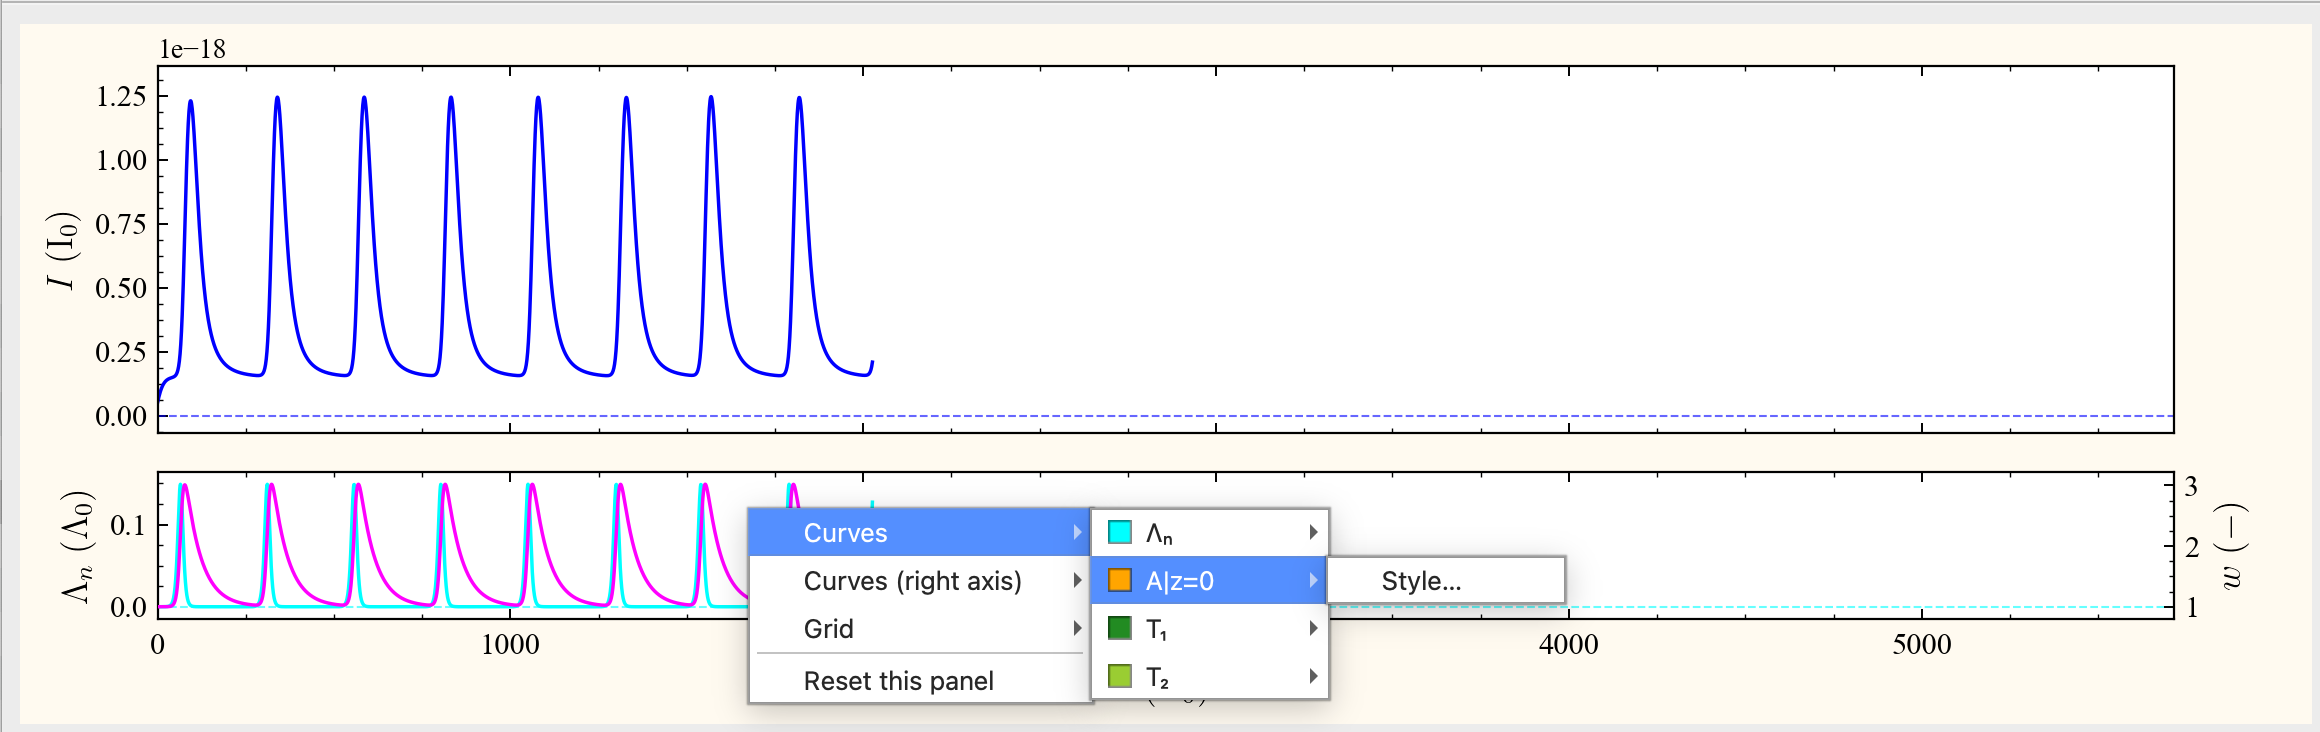
\includegraphics[width=\textwidth]{figures/plot_menu.png}
  \caption{Right-clicking the bottom panel: \menu{Curves} lists each curve with its colour, each with a \menu{Style...} entry.}
  \label{fig:plot-menu}
\end{figure}

% ══════════════════════════════════════════════════════════════════════════════
\section{Fit Mode}
\label{sec:fitmode}

Fit mode is used to compare the model with observed light curves one velocity component at a time.
Figure~\ref{fig:fit-mode} shows a data folder loaded: the toolbar is active, the top panel shows the
observed flux with the model, and the time axis is in days.
\begin{figure}[htbp]
  \centering
  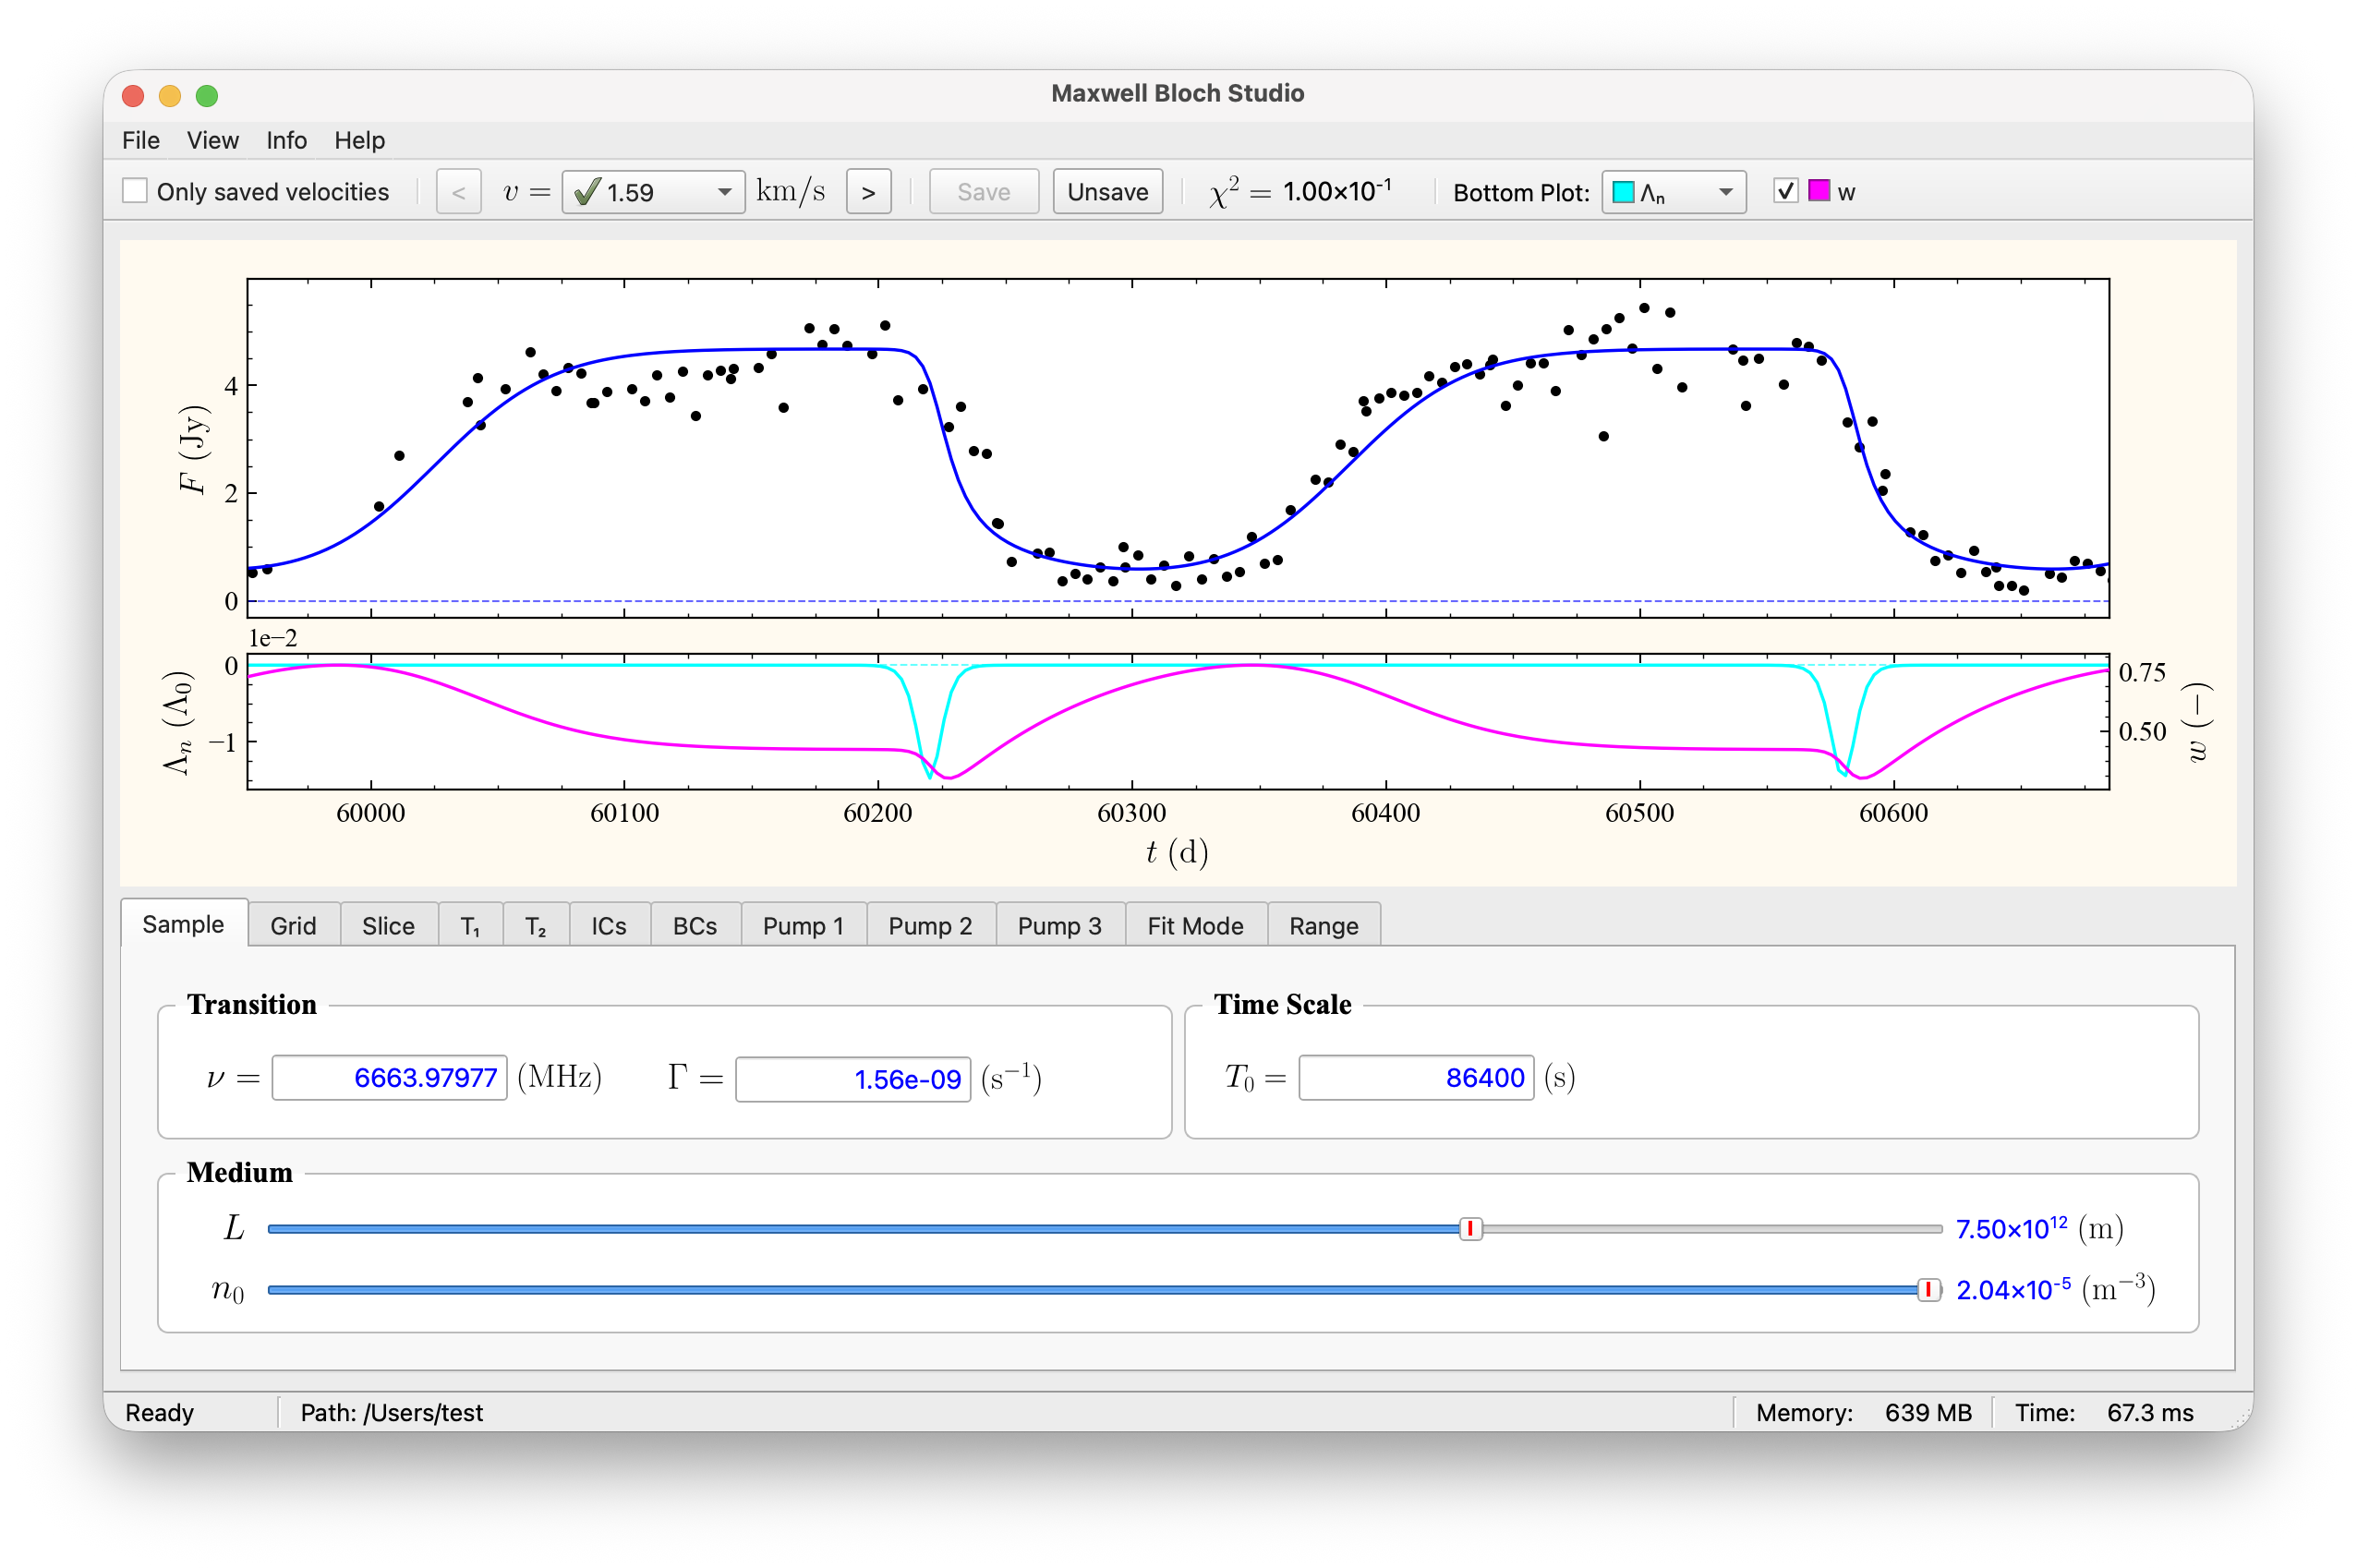
\includegraphics[width=\textwidth]{figures/fit_mode.png}
  \caption{Fit mode with a data folder loaded. The selected velocity component is saved (\checkmark), and $\chi^2$ shows the mismatch for it.}
  \label{fig:fit-mode}
\end{figure}

\subsection{Loading a Data Folder}

To enter fit mode:
\begin{enumerate}[noitemsep]
  \item choose \menu{File $\to$ Open Data Folder...} (\key{Ctrl+Shift+O}),
  \item select the folder containing the data files,
  \item if more than one period group is present, choose the desired period,
  \item review the import summary dialog.
\end{enumerate}

If matching saved parameters already exist in the folder, they are loaded automatically.

\subsubsection*{Expected File Naming}

The application expects filenames of the form
\begin{verbatim}
SourceName_v=12.3.txt
SourceName_p1_v=12.3.txt
\end{verbatim}
where the optional token \texttt{p1}, \texttt{p2}, \dots{} is a period label and \texttt{v=} denotes the velocity.

\subsubsection*{Folder Rules}

A valid data folder should satisfy the following conditions:
\begin{itemize}[noitemsep]
  \item all valid files belong to the same source,
  \item files are either all period-tagged or all non-period-tagged,
  \item each light-curve file is plain text,
  \item the app reads the \textbf{first two numeric columns} as time and flux,
  \item blank lines and lines beginning with \texttt{\#} are ignored.
\end{itemize}

\begin{warnbox}
\menu{File $\to$ Open Parameters...} is intended for standalone parameter snapshots, not for fit-mode source files.
Fit-mode parameter sets are loaded automatically from the selected data folder.
\end{warnbox}

\subsection{Velocity Navigation}

Once a data folder is open, the velocity toolbar becomes active.
You can:
\begin{itemize}[noitemsep]
  \item move to the previous or next component,
  \item choose a component directly from the drop-down list,
  \item filter the list with \textbf{Only saved velocities},
  \item save or unsave the current component.
\end{itemize}

Each velocity component has its own stored parameter state.

\subsection{Save and Unsave Behaviour}

In fit mode, pressing \textbf{Save} or using \key{Ctrl+S} saves the current velocity's parameters into a
single source-level JSON file in the loaded folder:
\begin{verbatim}
SourceName_params.json
SourceName_p1_params.json
\end{verbatim}
The file stores the saved states for all velocities in the selected source/period group.

The \textbf{Unsave} button removes the saved state of the current velocity from that file.

If a velocity has unsaved changes and you try to switch away from it, the app asks whether you want to
save, discard, or cancel the change.

\subsection{Mismatch Readout}

The toolbar shows a quantity labeled $\chi^2$.
Within the app, this is a \textbf{reduced $\chi^2$-like mismatch} computed over the currently visible data range.
It is useful as a quick comparison metric, but it is \textbf{not} a formal statistical reduced chi-square based on
measurement uncertainties.

\subsection{Closing Data}

Choose \menu{File $\to$ Close Data} (\key{Ctrl+W}) to leave fit mode and return to the default standalone state.
If there are unsaved changes, the app prompts before closing the folder.

% ══════════════════════════════════════════════════════════════════════════════
\newpage
\section{File Menu Reference}
The shortcuts below use Windows/Linux conventions. On macOS, replace \key{Ctrl} with \key{Cmd} and \key{Alt} with \key{Option}.

\begin{center}
\begin{tabular}{@{}lll@{}}
  \toprule
  Menu Item & Shortcut & Description \\
  \midrule
  Open Data Folder...        & \key{Ctrl+Shift+O} & Import a data folder and enter fit mode \\
  Recent Data Folders        & ---                & Reopen a recently used source folder \\
  Open Current Source Folder & \key{Ctrl+O}       & Open the active source folder in the file browser \\
  Open Parameters...         & \key{Ctrl+Shift+P} & Import a standalone parameter snapshot \\
  Close Data                 & \key{Ctrl+W}       & Close the loaded data folder \\
  Save Parameters            & \key{Ctrl+S}       & Save current parameters \\
  Save Parameters As...      & \key{Ctrl+Shift+S} & Save a standalone snapshot to a new file \\
  Save Parameters as Default & \key{Ctrl+Alt+S}   & Store the current state as the startup default \\
  Export Plot...             & \key{Ctrl+E}       & Export the current figure \\
  Quit                       & \key{Ctrl+Q}       & Exit the application \\
  \bottomrule
\end{tabular}
\end{center}

\begin{notebox}
In fit mode, \menu{Save Parameters As...} is disabled. The active save target is the source-level parameter file
inside the loaded data folder.
\end{notebox}

% ══════════════════════════════════════════════════════════════════════════════
\section{View Menu Reference}

\begin{center}
\begin{tabular}{@{}lll@{}}
  \toprule
  Menu Item & Shortcut & Description \\
  \midrule
  Show Slider Range & \key{Ctrl+Alt+R} & Show or hide slider range labels \\
  Reset Plot Style  & ---              & Return curve styles, grids, grid style and span style to their defaults \\
  \bottomrule
\end{tabular}
\end{center}

Grid lines, curve colours, line styles and the span style are set from the plot's right-click menu
(Section~\ref{sec:plot-style}).

% ══════════════════════════════════════════════════════════════════════════════
\section{Info and Help Menus}

\begin{center}
\begin{tabular}{@{}lll@{}}
  \toprule
  Menu Item & Shortcut & Description \\
  \midrule
  Data Summary        & \key{Ctrl+Alt+D} & Show source, period, velocity, and data ranges \\
  Scaling Formula     & \key{Ctrl+Alt+F} & Show the scaling expression used by the app \\
  Equations Reference & \key{Ctrl+Alt+E} & Open the bundled equations reference PDF \\
  Solver Step Viewer  & \key{Ctrl+Alt+V} & Open the interactive solver-step viewer \\
  User Guide          & \key{F1}         & Open the user guide PDF if available \\
  Use from Python     & ---              & Show the example script for your own scripts \\
  Check for Updates   & ---              & Ask PyPI whether a newer version exists \\
  About This App      & ---              & Show application and author information \\
  About Qt            & ---              & Show the Qt about dialog \\
  \bottomrule
\end{tabular}
\end{center}

The app also checks for a newer version a few seconds after it starts. When one exists, a notice
shows how to update and, below it, \textbf{What's new}: the release notes of every newer version,
newest first. \menu{Open Release Notes} opens all notes on GitHub. Without an internet connection
the check is skipped silently.

% ══════════════════════════════════════════════════════════════════════════════
\section{Exporting Plots}

Use \menu{File $\to$ Export Plot...} to save the current figure.

\begin{itemize}[noitemsep]
  \item \textbf{PDF:} exports the current plot on the first page and appends one or more text-report pages
  containing metadata and the current parameter values.
  \item \textbf{PNG / SVG:} exports the figure only.
\end{itemize}

The exported PDF also includes document metadata such as title, creator, and author name.

% ══════════════════════════════════════════════════════════════════════════════
\section{Saving and Loading Parameters}

\subsection{Saved JSON Structure}\label{sec:json}

Saved parameter snapshots use the structure
\begin{verbatim}
{
  "metadata": { ... },
  "config":   { ... },
  "params":   { ... }
}
\end{verbatim}
where:
\begin{itemize}[noitemsep]
  \item \texttt{metadata} stores version, save time, username, and mode information,
  \item \texttt{config} stores widget/configuration state,
  \item \texttt{params} stores the current parameter values.
\end{itemize}

In fit mode, the \texttt{params} section stores the saved values for all saved velocities in the source/period group.

The \texttt{solve.sample} entry stores only the physical sample values
($\nu$, $\Gamma$, $T_0$, $L$, $n_0$, in SI units). The derived quantities such as
$\eta$ and $\theta_0$ are computed from them whenever the model is solved; values
of $\eta$ and $\theta_0$ found in files from older versions are ignored.

\subsection{App Defaults}

The command \menu{File $\to$ Save Parameters as Default} stores the current standalone state in the platform's
persistent application settings using Qt's \texttt{QSettings}. On later launches, the app restores these saved defaults
instead of the factory defaults.

% ══════════════════════════════════════════════════════════════════════════════
\section{Using the Solver from Python}\label{sec:python}

Parameter files saved by the app can be solved in your own scripts, for example
to run many cases without the window. Install the app with \texttt{pip} in the
Python environment you use (a \texttt{pipx} installation is kept separate from
your own Python):
\begin{verbatim}
pip install maxwell-bloch-studio
\end{verbatim}

A minimal script:
\begin{verbatim}
import mbstudio

f = mbstudio.ParamsFile("run_1.json")     # a file saved by the app
params = f.params()                       # a fresh dictionary, safe to change
params["solve.sample"]["l"] = 1.0e13      # change any value
res = mbstudio.solve(params)              # same numbers as the app

res["time"]             # time grid
res["intensity"][-1]    # intensity at the exit of the medium
\end{verbatim}

\begin{itemize}[noitemsep]
  \item \texttt{ParamsFile} also gives \texttt{metadata}, \texttt{app\_version} and, for the
  parameter file of a data folder, the list \texttt{velocities}; choose one component
  with \texttt{f.params(12.3)}.
  \item \texttt{params} is the dictionary stored under \texttt{"params"} in the file
  (Section~\ref{sec:json}). Files from older versions are converted automatically.
  \item $\eta$ and $\theta_0$ are computed from the sample values
  ($\nu$, $\Gamma$, $T_0$, $L$, $n_0$), as in the app;
  \texttt{mbstudio.scaling(nu=..., gamma=..., t0=..., l=..., n0=...)} returns them
  together with the other derived quantities.
  \item The result holds \texttt{time}, \texttt{intensity} and \texttt{w} (one row per
  stored $z$ plane, from the entrance to the exit), \texttt{lambda\_n} (pump),
  \texttt{A0} (boundary field), \texttt{t1} and \texttt{t2}, in the solver's dimensionless
  units. The flux scaling and offsets of the Fit Mode tab are not applied.
\end{itemize}

\begin{notebox}
\menu{Help $\to$ Use from Python...} shows a commented example script that lists every
parameter and result key; copy it or save it as a \texttt{.py} file to start from.
\end{notebox}

\begin{figure}[htbp]
  \centering
  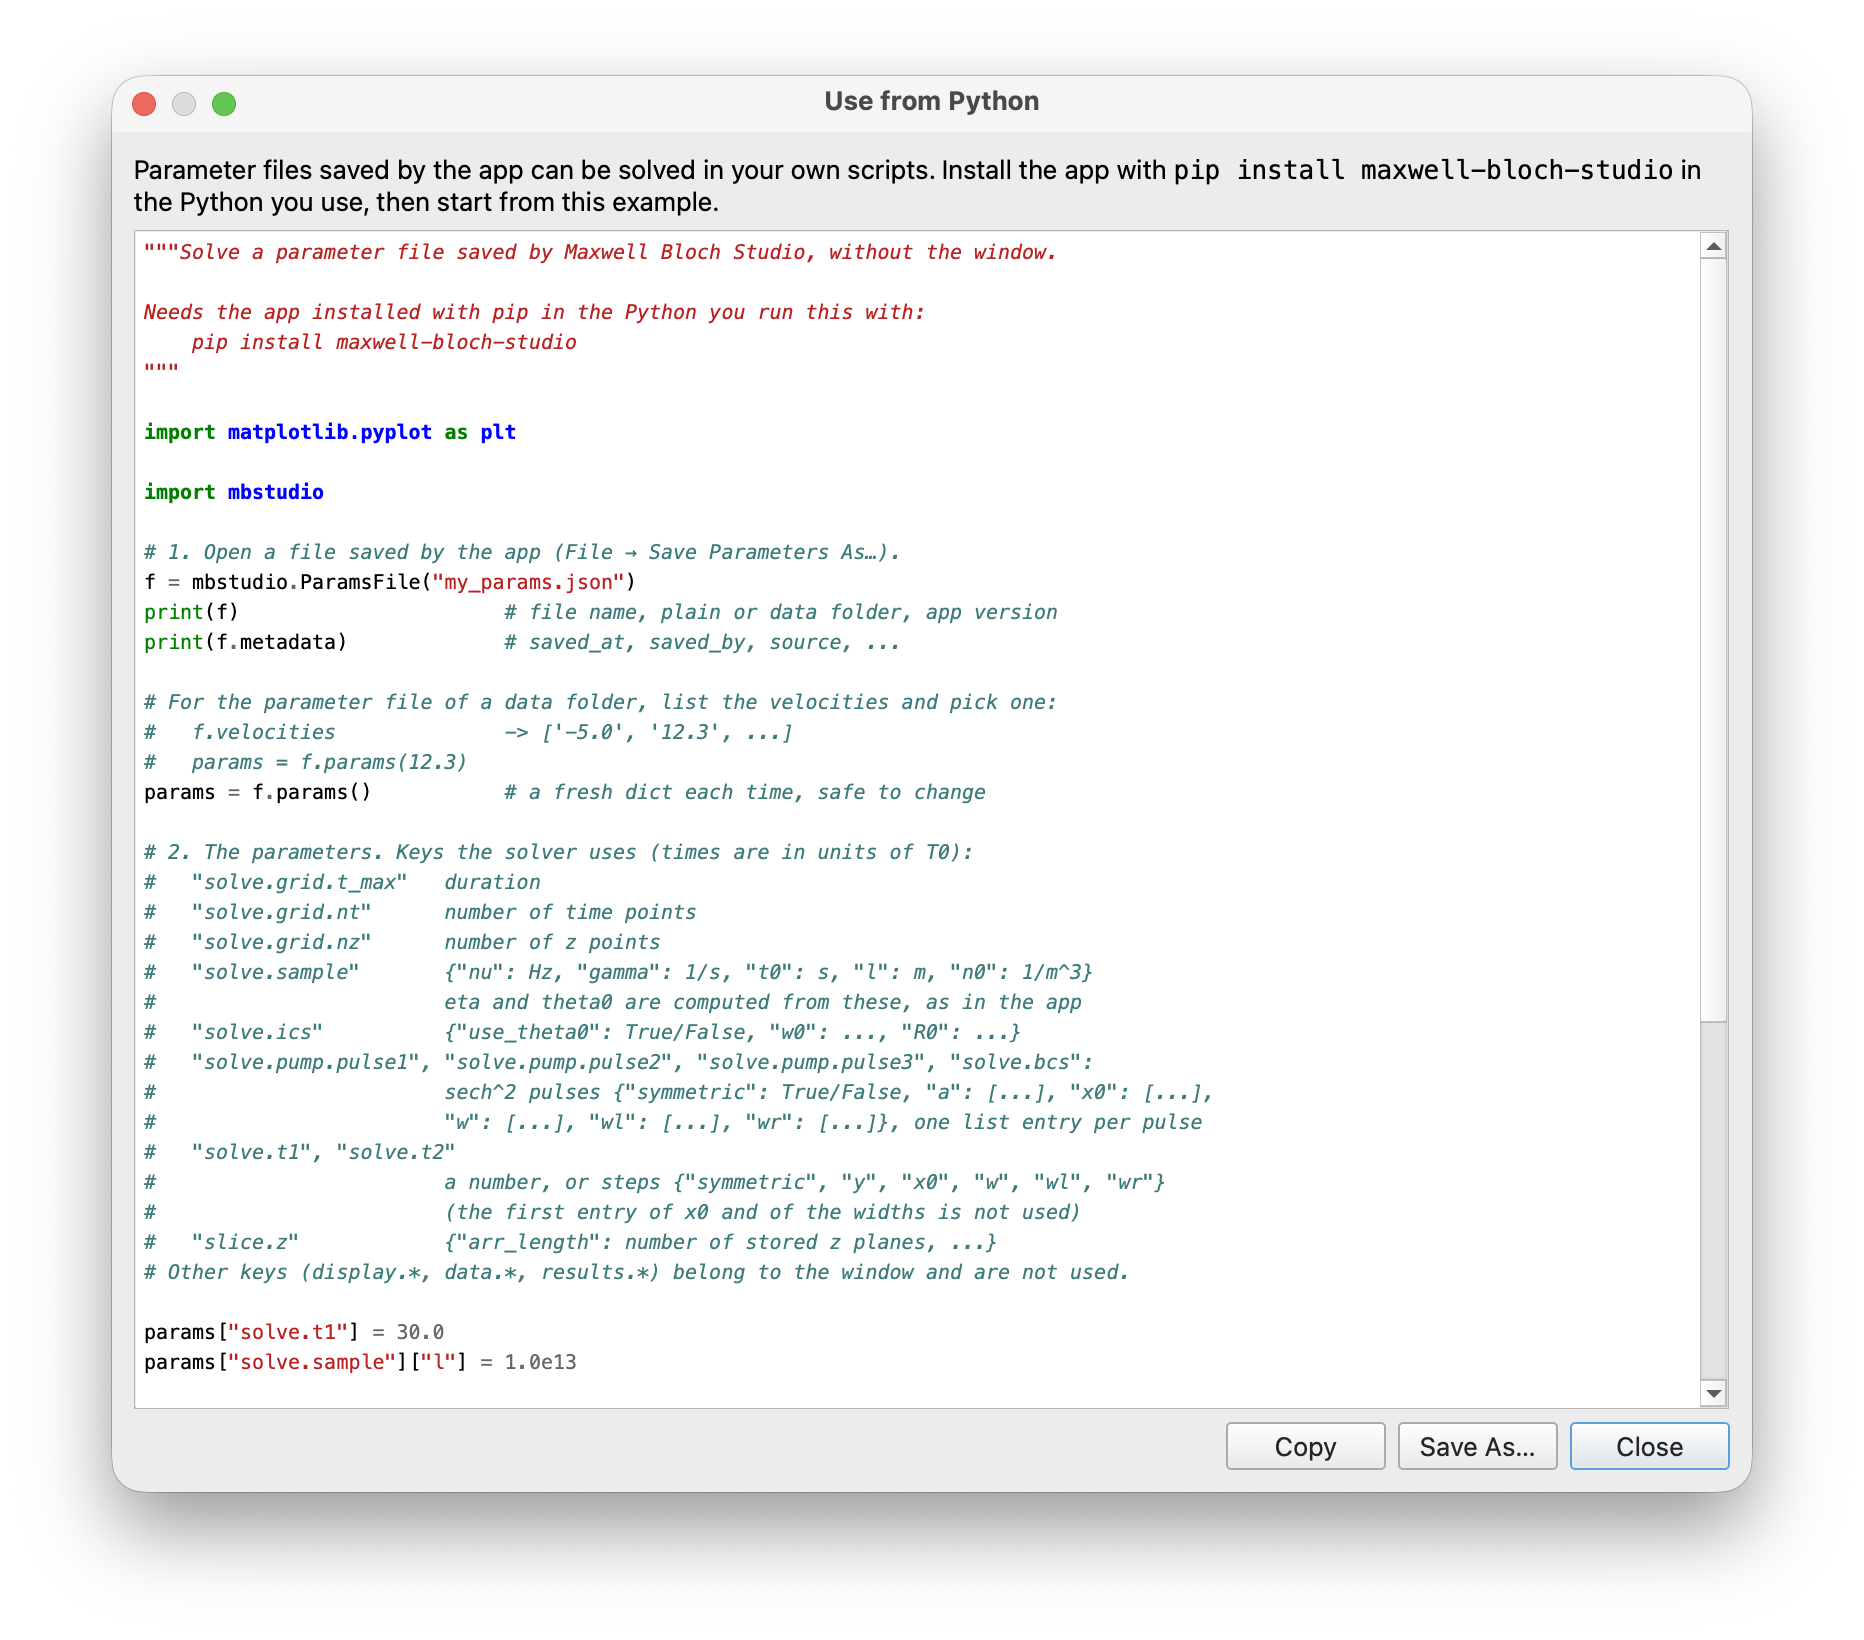
\includegraphics[width=0.8\textwidth]{figures/python_dialog.png}
  \caption{\menu{Help $\to$ Use from Python...}: the example script, ready to copy or save.}
  \label{fig:python-dialog}
\end{figure}

The numerical solver itself is the separate package \texttt{mbsolver}
(\texttt{pip install mbsolver}), for building parameters directly in code.

% ══════════════════════════════════════════════════════════════════════════════
\section{Typical Workflows}

\subsection{Standalone Simulation Workflow}

\begin{enumerate}
  \item Launch the application.
  \item Set the physical sample parameters in \tab{Sample}.
  \item Adjust the numerical resolution in \tab{Grid} if needed.
  \item Choose the initial state in \tab{ICs}.
  \item Set the relaxation times in \tab{T\textsubscript{1}} and
        \tab{T\textsubscript{2}}, either as constants or as step profiles.
  \item Define the boundary field in \tab{BCs}.
  \item Add up to three pump contributions in \tab{Pump 1}, \tab{Pump 2},
        and \tab{Pump 3}.
  \item Inspect different propagation slices in \tab{Slice}.
  \item Use \tab{Range} to zoom the displayed region.
  \item Export the plot or save the parameters when satisfied.
\end{enumerate}

\subsection{Observational Fitting Workflow}

\begin{enumerate}
  \item Open a data folder with \menu{File $\to$ Open Data Folder...}.
  \item Select a velocity component from the toolbar.
  \item Use \tab{Fit Mode} to choose the correct data time unit and apply any needed offsets.
    \item Adjust the physical and driving parameters in \tab{Sample},
        \tab{T\textsubscript{1}}, \tab{T\textsubscript{2}}, \tab{ICs},
        \tab{BCs}, and the pump tabs.
  \item Use the fit controls to align the model in time and scale it vertically.
  \item Monitor the $\chi^2$-style mismatch as a quick diagnostic.
  \item Save the current velocity.
  \item Repeat for the remaining velocities.
\end{enumerate}

% ══════════════════════════════════════════════════════════════════════════════
\section{Troubleshooting}

\begin{description}[leftmargin=2em,style=nextline]
  \item[The plot does not seem to change after I edit a value.]\
  Solver parameters under \texttt{solve.*} trigger a new solve. Pure display parameters such as
  range settings, selected slice index, or fit offsets may update the display without re-solving.

  \item[Open Parameters refuses one of my saved JSON files.]\
  That file is probably a fit-mode source parameter file. Load the corresponding data folder instead;
  the app will read that file automatically.

  \item[The imported folder is rejected.]\
  Check the filename pattern and make sure the folder contains only one source name and is not mixing
  period-tagged and non-period-tagged data files.

  \item[The solver becomes slow.]\
  Large values of $N_t$ and $N_z$ increase compute time. The first solve after launch may also be slower
  because the JIT-compiled kernels are being prepared.

  \item[The mismatch value is blank.]\
  This happens when there is no loaded data, no visible overlap between the plotted data and model,
  or no valid interpolated comparison range.

  \item[The PDF export contains extra pages.]\
  This is expected. PDF export includes a report section with metadata and parameters in addition to the figure page.
\end{description}

\vfill
\begin{center}
  \small\color{gray}
  \AppName \, v\AppVersion \quad|\quad \AppAuthor \quad|\quad
  \href{mailto:\AppEmail}{\AppEmail}
\end{center}

\end{document}
